\documentclass[aspectratio=169,sn-mathphys-num]{beamer}

\usepackage{fontspec}
\usepackage{unicode-math}
\usepackage{graphicx}
\usepackage[dvipsnames]{xcolor}
\usepackage[sorting=none]{biblatex}
\usepackage{ragged2e}
\usepackage{setspace}
\usepackage{bookmark}
\usepackage{siunitx}
\usepackage{mhchem}
\usepackage{braket}
\usepackage{tikz}

\addbibresource{../references.bib}

\usetheme[numbering=counter, progressbar=frametitle, background=light]{metropolis}

\usecolortheme{dove}
\definecolor{primary}{RGB}{88, 24, 124}
\definecolor{secondary}{RGB}{0, 168, 150}

\setbeamercovered{transparent}
\setbeamercolor{frametitle}{fg=white, bg=primary}
\setbeamercolor{progress bar}{fg=secondary}
\setbeamerfont{frametitle}{size=\large, series=\bfseries}
\setbeamerfont{title}{size=\LARGE, series=\bfseries}
\setbeamercolor{alerted text}{fg=secondary}
\setbeamercolor{block title}{fg=primary}
\setbeamercolor{block body}{bg=white}

\setstretch{1.1}

\setmainfont{Fira Sans}
\setmathfont{TeX Gyre Pagella Math}

\newcommand{\Tr}{\mathrm{Tr}}

\title{Quantum Entanglement}
\subtitle{Spooky and Hidden}
\author{Avila, Herrera, Rodríguez}
\institute{Universidad Distrital Francisco José de Caldas}
\date{\today}

\begin{document}

\begin{frame}
	\titlepage
\end{frame}

\section{EPR Debate}
% --- SLIDE 1: Einstein's Realism ---
\begin{frame}{The Clash of Titans: Einstein's Realism}

  \begin{columns}
    % Column for text
    \begin{column}{0.5\textwidth}
      \begin{itemize}[<+->] % Items appear one by one
        \item \textbf{Deterministic View:} The universe is knowable and orderly.
        \item \textbf{Objective Reality:} Physical properties exist independently of measurement.
        \item \textbf{No Fundamental Randomness:} Probability is not intrinsic to nature.
      \end{itemize}
    \end{column}

    % Column for image
    \begin{column}{0.5\textwidth}
      \begin{center}
        \begin{figure}
          \centering
          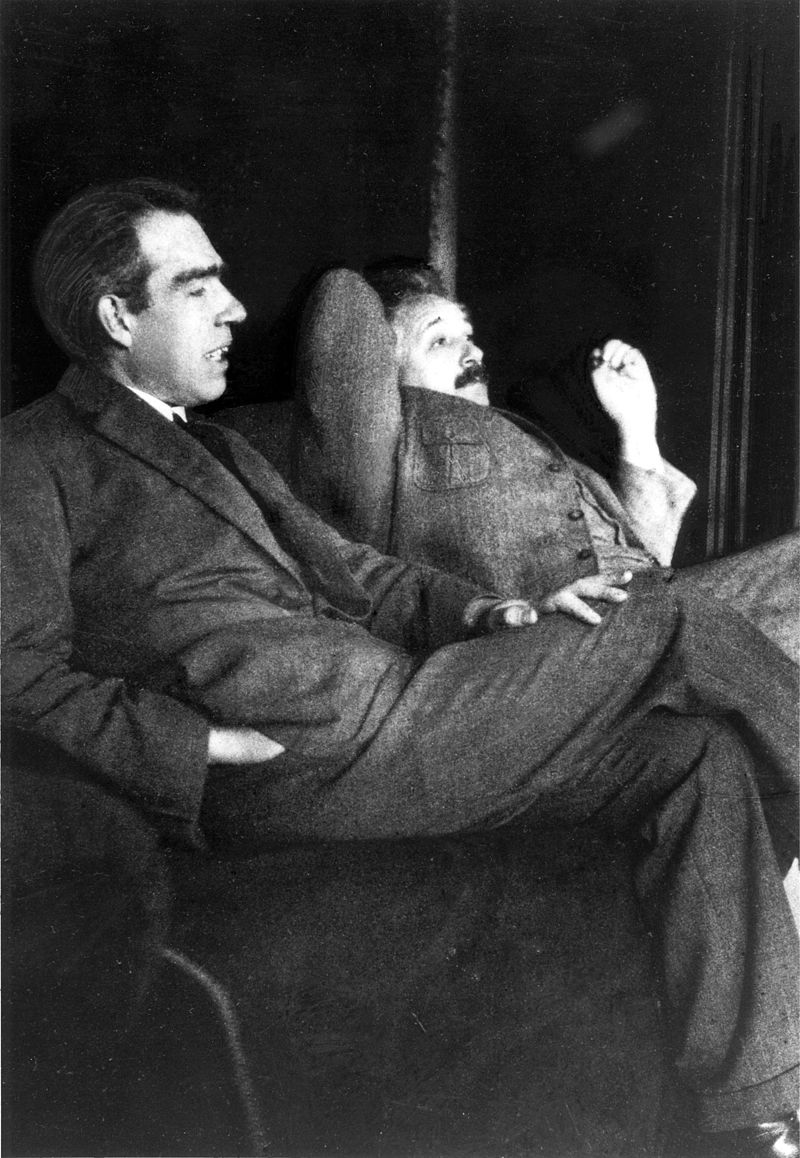
\includegraphics[width=0.5\linewidth]{images/Borhn-Einstein.jpg}
          \caption{Niels Bohr with Albert Einstein at Paul Ehrenfest's home in Leiden \cite{IBorhEinstein}.}
        \end{figure}
      \end{center}
    \end{column}
  \end{columns}

\end{frame}

% --- SLIDE 2: The EPR Paradox ---
\begin{frame}{The EPR Paradox: A Challenge in 1935}

  \begin{columns}
    % Column for text
    \begin{column}{0.55\textwidth} % Wider for the paper's text
      \begin{block}{The Seminal Paper}
        \begin{itemize}[<+->]
          \item In 1935, Einstein, Podolsky, and Rosen published a key paper.
          \item A ``frontal assault'' on the conceptual foundations of quantum mechanics.
          \item Their goal: To question whether the quantum description of reality is \emph{complete}.
          \item The title: ``Can Quantum-Mechanical Description of Physical Reality Be Considered Complete?''.
        \end{itemize}
      \end{block}
    \end{column}

    % Column for image
    \begin{column}{0.45\textwidth} % Narrower for the image
      \begin{center}
       \begin{figure}
        \centering
        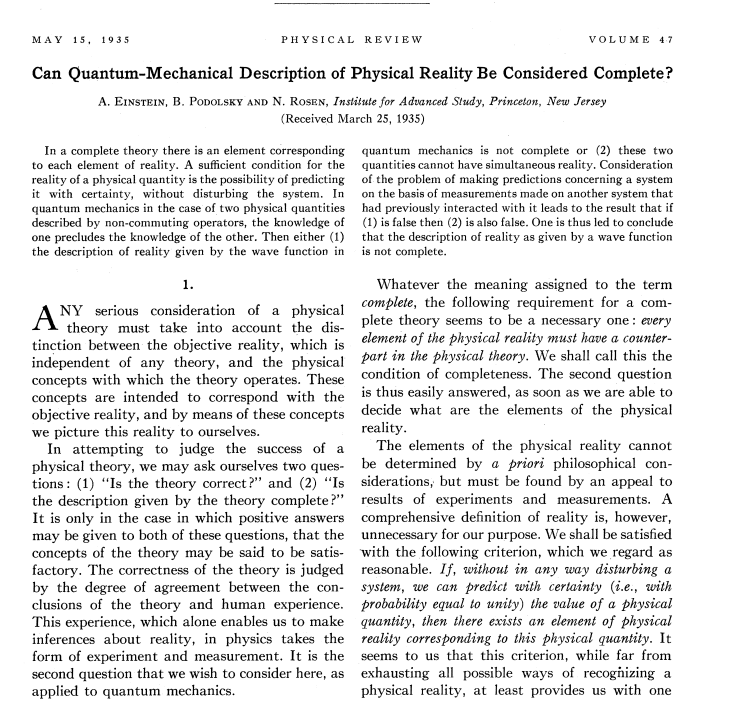
\includegraphics[width=0.5\linewidth]{images/EPR-articulo.png}
        \caption{Paper: Can Quantum-Mechanical Description of Physical Reality Be Considered Complete? \cite{Einstein1935}}
      \end{figure}
      \end{center}
    \end{column}
  \end{columns}

\end{frame}

% --- SLIDE 3: EPR's Criterion of Reality ---
\begin{frame}{The EPR Criterion of Reality}

  \begin{block}{The ``rule'' to define an element of reality}
    To formalize their attack, EPR introduced an explicit and, seemingly, irrefutable criterion:
  \end{block}
  \pause % Wait for a click to show the quote

  \begin{quote}
    ``If, without in any way disturbing a system, we can predict with certainty (i.e., with probability equal to unity) the value of a physical quantity, then there exists an element of physical reality corresponding to this physical quantity.''
  \end{quote}

\end{frame}

% --- SLIDE 4: Violation of the Criterion ---
\begin{frame}{Violation of the Criterion: Position and Momentum}

  \begin{block}{Example with a state $\psi = e^{(2\pi i/h)p_0x}$}
    \begin{itemize}[<+->] % Items appear one by one
      \item When applying the momentum operator ($p$), we get an exact value:
      $$ p\psi = \left(\frac{h}{2\pi i}\frac{\partial}{\partial x}\right)\psi = p_0\psi $$
      It is concluded that the momentum, $p_0$, is an \textbf{element of reality}.
      \item However, when applying the position operator ($x$), an exact value is not obtained:
      $$ x\psi \neq \text{constant} \cdot \psi $$
      We can only calculate the \textbf{probability} of finding the particle in an interval $[a, b]$, which turns out to be $P(a,b) = b-a$.
    \end{itemize}
  \end{block}

\end{frame}

% --- SLIDE 5: The EPR Conclusion ---
\begin{frame}{The EPR Conclusion}

  \begin{alertblock}{The Fundamental Dichotomy}
    From the previous example, it follows that there are only two possibilities:
    \begin{enumerate}[<+->] % List items appear one by one
        \item Either the quantum-mechanical description of reality given by the wave function \textbf{is not complete}.
        \item Or when the operators for two physical quantities do not commute, the two quantities \textbf{cannot have simultaneous reality}.
    \end{enumerate}
  \end{alertblock}
\end{frame}

% --- SLIDE 6: The Principle of Locality ---
\begin{frame}{The Principle of Locality}

  \begin{block}{A fundamental idea in physics}
    \begin{itemize}[<+->] % Items appear one by one
      \item An object can only be directly influenced by its \textbf{immediate surroundings}.
      \item Any influence at a distance cannot be instantaneous; it must propagate at a finite speed, not exceeding the speed of light ($c$).
      \item For Einstein, locality was a sacred axiom. Its violation would imply the disintegration of the universe's \textbf{causal structure} (cause-and-effect).
    \end{itemize}
  \end{block}

\end{frame}

% --- SLIDE 7: The EPR Thought Experiment ---
\begin{frame}{The EPR Thought Experiment}

  \begin{columns}[T] % Align columns at the top
    % Column for text
    \begin{column}{0.6\textwidth}
      \begin{block}{The two-particle system}
        \begin{itemize}[<+->]
          \item A system of two particles is prepared in an entangled state and then separated by a large distance.
          \item \textbf{Option 1:} If Alice measures the \textbf{momentum} of her particle, she can predict with certainty the momentum of Bob's particle.
          \item \textbf{Option 2:} If Alice measures the \textbf{position}, she can predict with certainty Bob's position.
          \item \textbf{Partial Conclusion:} Both the position and momentum of Bob's particle must be ``elements of reality''.
        \end{itemize}
      \end{block}
    \end{column}

    % Column for image
    \begin{column}{0.4\textwidth}
      \begin{figure}
        \centering
        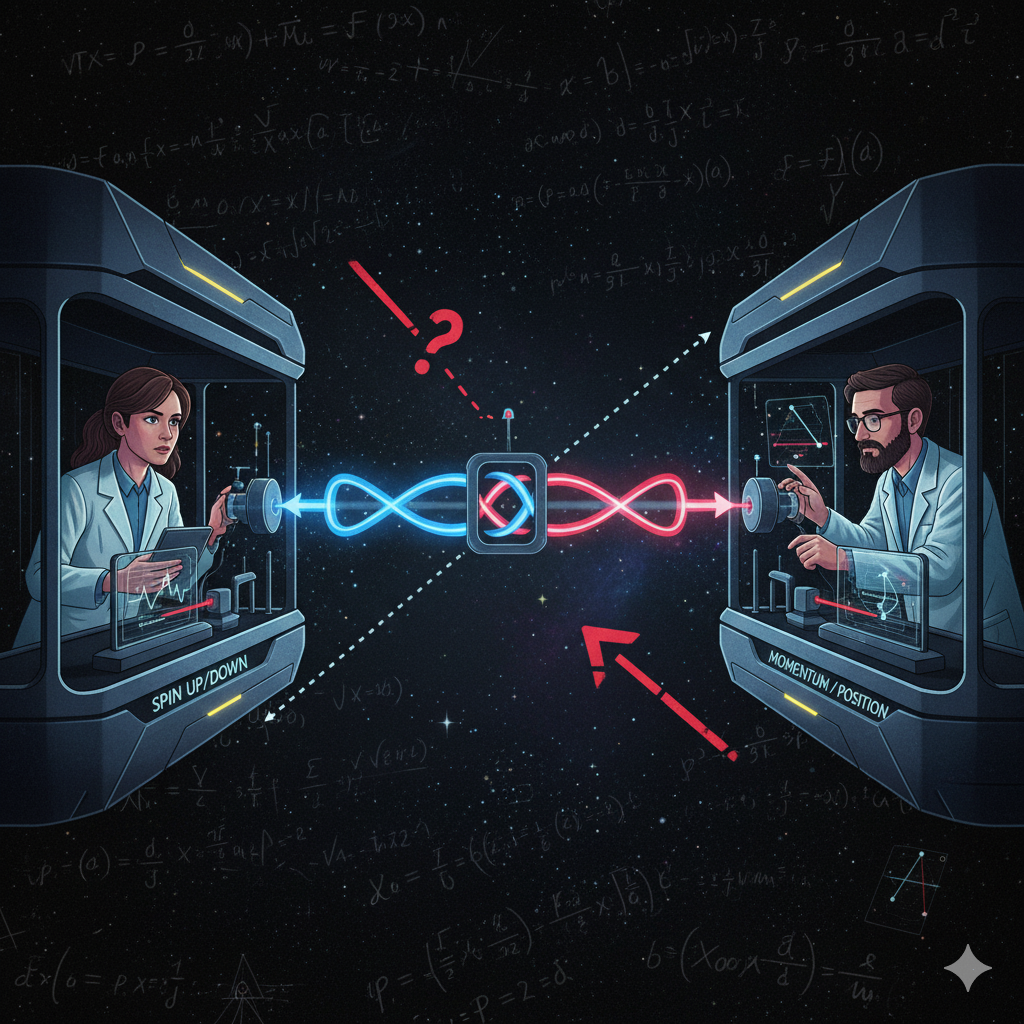
\includegraphics[width=\linewidth]{images/epr_experiment.png}
        \caption{Alice and Bob measure entangled particles separated by a large distance \cite{Google2025_AliceBob}.}
      \end{figure}
    \end{column}
  \end{columns}

\end{frame}

% --- SLIDE 8: The Contradiction and EPR's Conclusion ---
\begin{frame}{The Contradiction and EPR's Conclusion}

  \begin{block}{The Conflict with Quantum Mechanics}
    \begin{itemize}[<+->]
      \item The conclusion that Bob's particle has a definite position and momentum \textbf{simultaneously}...
      \item ...is in direct conflict with the \textbf{Heisenberg Uncertainty Principle}, which forbids it.
    \end{itemize}
  \end{block}

  \begin{alertblock}<3->{The EPR Conclusion}
    Faced with this dilemma, if local realism is correct, the only possible conclusion is that:
    \begin{itemize}[<+->]
      \item The description of reality provided by the wave function must be \textbf{incomplete}.
      \item There must be an underlying theory (``hidden variables'') that provides a complete description.
    \end{itemize}
  \end{alertblock}

\end{frame}

% --- SLIDE 9: Bohr's Response ---
\begin{frame}{Bohr's Response: The Principle of Complementarity}

  \begin{columns}[T] % Align columns at the top
    % Column for text
    \begin{column}{0.55\textwidth}
      \begin{block}{Mutually Exclusive, Yet Necessary Concepts}
        \begin{itemize}[<+->] % Items appear one by one
          \item Complementarity posits that pairs of classical concepts are necessary for a complete description.
          \item But they are \textbf{mutually exclusive} in any single experiment.
          \item They are not contradictory properties of the object, but complementary aspects of a \textbf{phenomenon} revealed by incompatible experimental arrangements.
        \end{itemize}
    \end{block}
    \end{column}

    % Column for image
    \begin{column}{0.45\textwidth}
      \begin{figure}
        \centering
        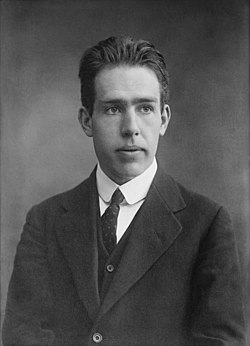
\includegraphics[width=\linewidth, height=0.7\textheight, keepaspectratio]{images/NielsBohr.jpg}
        \caption{Niels Bohr \cite{IBohr}.}
      \end{figure}
    \end{column}
  \end{columns}

\end{frame}

% --- SLIDE 10: Is Quantum Mechanics Complete? Bohr's View ---
\begin{frame}{Is Quantum Mechanics Complete? Bohr's View}

  \begin{block}{Radical Revision of Physical Reality}
    \begin{itemize}[<+->]
      \item The experimenter's ``freedom of choice'' does not reveal pre-existing realities, but rather \textbf{creates different experimental conditions} and phenomena.
      \item Quantum mechanics is \textbf{complete} because it correctly and exhaustively describes the results of \emph{every possible, well-defined experiment}.
      \item Bohr compares this revision of physical reality to the modification of ideas about the absolute character of phenomena introduced by the \textbf{Theory of Relativity}.
      \item This philosophical debate was crucial and led to \textbf{Bell's Theorem} and subsequent experiments, turning EPR into a testable question.
    \end{itemize}
  \end{block}

\end{frame}

% --- SLIDE 11: Schrödinger's Response ---
\begin{frame}{Schrödinger's Response: The Birth of ``Entanglement''}

  \begin{columns}[T] % Align columns at the top
    % Column for text
    \begin{column}{0.6\textwidth}
      \begin{block}{Context and the Essence of the New Physics}
        \begin{itemize}[<+->]
          \item A few months after EPR, Schrödinger published his response: ``Discussion of Probability Relations between Separated Systems''.
          \item He demonstrated a deep understanding and took the EPR argument to its most extreme conclusions.
          \item He understood that the phenomenon was not an anomaly, but \textbf{the characteristic trait of quantum mechanics}.
          \item He coined the term \textbf{``Entanglement'' (Verschränkung)}.
        \end{itemize}
    \end{block}
\end{column}

    % Column for image
    \begin{column}{0.4\textwidth}
      \begin{figure}
        \centering
        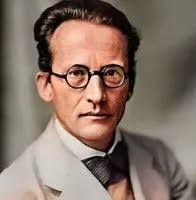
\includegraphics[width=\linewidth, height=0.7\textheight, keepaspectratio]{images/schrodinger.jpeg}
        \caption{Erwin Schrödinger \cite{Anon1933_Schrodinger}.}
      \end{figure}
    \end{column}
  \end{columns}

\end{frame}

% --- SLIDE 12: Steering ---
\begin{frame}{``Steering'' and the Schmidt Decomposition}

  \begin{block}{The most unsettling aspect of Entanglement}
    \begin{itemize}[<+->]
      \item Schrödinger identified an experimenter's ability to \textbf{``steer'' (steuern)} the state of a distant system.
      \item This is achieved through the local choice of measurement.
      \item He described it as ``rather discomforting that the theory allows a system to be steered... at the whim of the experimenter, even though they have no access to it''.
      \item Rigorously demonstrated with a mathematical formalism: the \textbf{Schmidt decomposition}.
    \end{itemize}
  \end{block}

\end{frame}

% --- SLIDE 13: Bohr vs. Schrödinger ---
\begin{frame}{Bohr vs. Schrödinger: Two Approaches to the Paradox}

  \begin{block}{Fundamental Differences in the Response to EPR}
    \begin{itemize}[<+->]
      \item \textbf{Bohr:} Offered a philosophical framework (complementarity) to \emph{dissolve the paradox}, declaring that EPR's questions were ill-posed.
      \item \textbf{Schrödinger:} Accepted the validity of EPR's questions and delved into the unsettling answers the theory provided, seeking to \emph{intensify the paradox}.
    \end{itemize}
  \end{block}

  \begin{alertblock}<3->{Schrödinger's Key Contributions}
    \begin{itemize}[<+->]
      \item \textbf{Named and defined the central concept:} He coined the term ``entanglement''.
      \item \textbf{Identified its most powerful manifestation:} The concept of ``steering,'' which captured the essence of non-locality.
      \item \textbf{Proved its generality with mathematical rigor:} He extended the EPR argument to all observables, showing its structural nature.
    \end{itemize}
  \end{alertblock}

\end{frame}


\section{Bohm-Aharonov}
% --- SLIDE 14: Bohm & Aharonov ---
\begin{frame}{Bohm \& Aharonov: Simplifying EPR}

  \begin{columns}[T]
    \begin{column}{0.6\textwidth}
      \begin{block}{A clearer, more experimental approach}
        \begin{itemize}[<+->]
          \item In 1951, \textbf{David Bohm} reformulated the EPR paradox in a conceptually clearer way.
          \item Together with \textbf{Yakir Aharonov} (in 1957), they simplified the example from continuous variables to the \textbf{discrete variable of spin}.
          \item This made the thought experiment much more \textbf{amenable to experimental verification}.
        \end{itemize}
      \end{block}
    \end{column}

    \begin{column}{0.4\textwidth}
      \begin{figure}
        \centering
        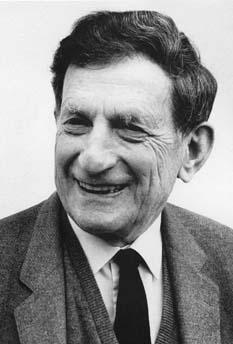
\includegraphics[width=\linewidth, height=0.7\textheight, keepaspectratio]{images/David_Bohm.jpg}
        \caption{David Bohm \cite{Anon_Bohm}.}
      \end{figure}
    \end{column}
  \end{columns}
\end{frame}

% --- SLIDE 15: The Spin Singlet State ---
\begin{frame}{The Spin Singlet State}
  \begin{columns}[T]
    \begin{column}{0.5\textwidth}
      \begin{block}{An example with spin-1/2 particles}
        \begin{itemize}[<+->]
          \item Consider a molecule with total spin zero that decays into two atoms (A and B) with spin 1/2.
          \item It is an \textbf{entangled} state where the total spin is zero, regardless of the measurement axis.
        \end{itemize}
      \end{block}
      \vspace{0.5em}
      The entangled wave function:
      $$ {\Psi} = \frac{1}{\sqrt{2}} \left( \Psi_{+}{(1)} \Psi_{-}{(2)} - \Psi_{-}{(1)} \Psi_{+}{(2)} \right) $$
    \end{column}

    \begin{column}{0.5\textwidth}
      \begin{figure}
        \centering
        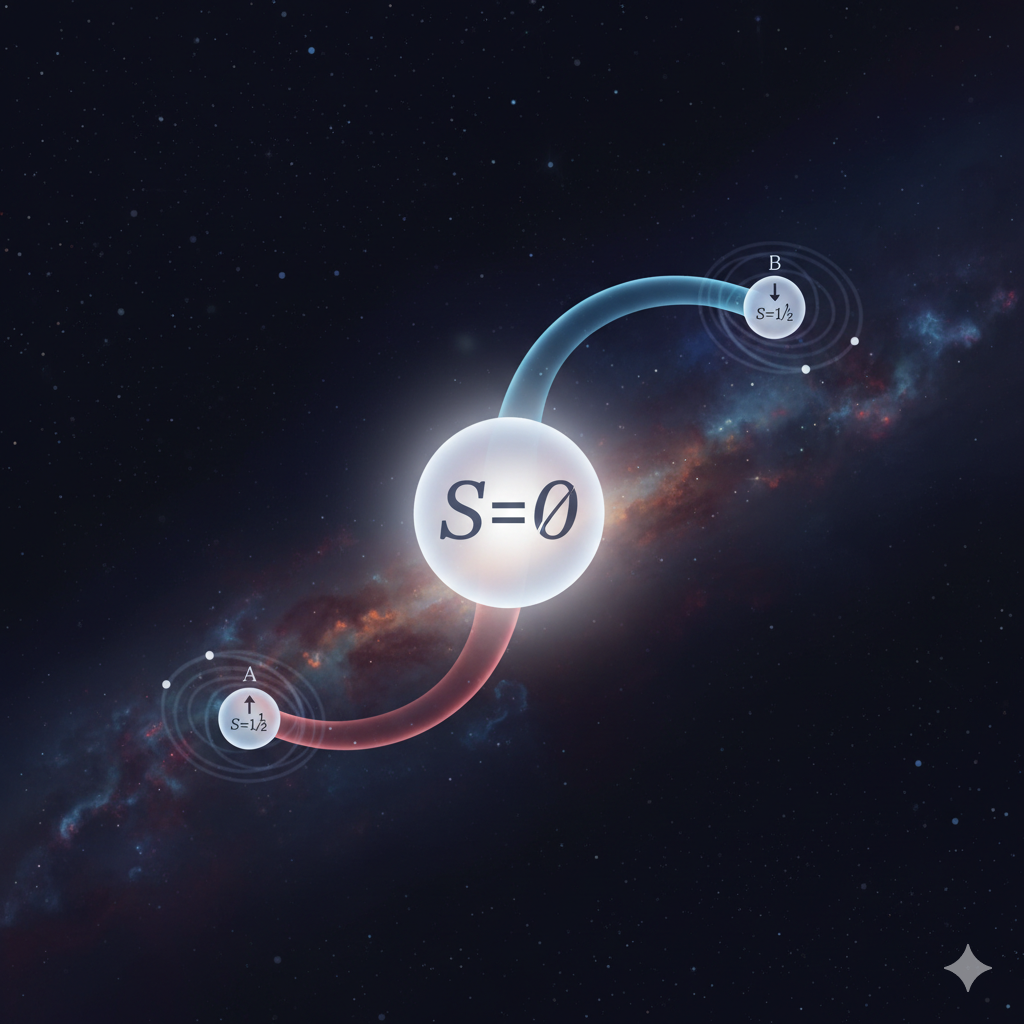
\includegraphics[height=0.7\textheight, keepaspectratio]{images/spin.png}
        \caption{A source emits two entangled particles with opposite spin \cite{Google2025_Entangled}.}
      \end{figure}
    \end{column}
  \end{columns}
\end{frame}

% --- SLIDE 16: Classical vs. Quantum ---
\begin{frame}{The Core of the Paradox: Classical vs. Quantum}

  \begin{columns}[T]
    \begin{column}{0.5\textwidth}
      \begin{alertblock}{Classical Interpretation (Local Realism)}
        \begin{itemize}[<+->]
          \item The atoms have \textbf{pre-existing} and perfectly anti-correlated spin vectors.
          \item The measurement on A only \textbf{reveals} an already existing property.
          \item There is no instantaneous influence at a distance; the correlation was established locally at the source.
        \end{itemize}
      \end{alertblock}
    \end{column}

    \begin{column}{0.5\textwidth}
      \begin{block}{Quantum Interpretation}
        \begin{itemize}[<+->]
          \item A particle's spin state is \textbf{not defined until it is measured}.
          \item The choice to measure A's spin \textbf{realizes} its value, and due to entanglement, simultaneously realizes the opposite value for B.
          \item This happens \textbf{instantaneously}, despite the distance, seemingly violating locality.
        \end{itemize}
      \end{block}
    \end{column}
  \end{columns}

  \uncover<7->{
    \textbf{Key conclusion:} Quantum uncertainty in entangled systems is an intrinsic property of the \textbf{non-separable correlations} that define the state of the system as a whole.
  }

\end{frame}

% --- SLIDE 17: Alternative Hypothesis ---
\begin{frame}{The Alternative Hypothesis: Entanglement Breaking}

  \begin{block}{Entanglement that ``decays'' with distance}
    \begin{itemize}[<+->]
      \item The idea is raised that the quantum many-body formulation \textbf{might not be valid} for widely separated particles.
      \item The proposal suggests that entanglement is a phenomenon that \textbf{decreases with distance}.
      \item An alternative \textbf{``classical'' state} is proposed for the system after separation.
    \end{itemize}
  \end{block}
  \uncover<4->{ % The equation appears after the points
    \justifying
    \vspace{0.5em}
    Alternative state (statistical mixture):
    $$ {\Psi} =  \Psi_{+\theta,\phi}{(1)} \Psi_{-\theta,\phi}{(2)}  $$
  }

\end{frame}

% --- SLIDE 18: Consequences and Difference ---
\begin{frame}{Consequences: Quantum Superposition vs. Classical Mixture}

  \begin{block}{Implications of the Breaking Hypothesis}
    \begin{itemize}[<+->]
      \item \textbf{Avoidance of the EPR Paradox:} It restores local realism; the measurement on A only reveals a pre-existing spin direction.
      \item \textbf{Violation of Angular Momentum Conservation:} In individual events, total angular momentum would not be conserved (but it would on average).
      \item This pre-existing spin direction acts as a \textbf{``hidden variable''}.
    \end{itemize}
  \end{block}

  \begin{alertblock}{Crucial Difference: Quantum Superposition vs. Statistical Mixture}
    \begin{itemize}[<+->]
      \item \textbf{Quantum Superposition (Entanglement):} Maintains perfect correlations in \textbf{any} measurement basis.
      \item \textbf{Classical Statistical Mixture:} Only exhibits perfect correlations in the basis defined by the hidden variable.
    \end{itemize}
  \end{alertblock}

\end{frame}

% --- SLIDE 19: Photon Polarization Analogue ---
\begin{frame}{An Experimental Analogue: Photon Polarization}

  \begin{columns}[T]
    \begin{column}{0.6\textwidth}
      \begin{block}{From Spin to Polarization}
        \begin{itemize}[<+->]
          \item A more viable analogue is proposed: the \textbf{polarization} of photons from \textbf{positron-electron annihilation}.
          \item \textbf{Conservation Laws:} Due to conservation of angular momentum and parity, the two emitted photons must have mutually \textbf{perpendicular} polarizations.
        \end{itemize}
      \end{block}
      \vspace{0.5em}
      Wave function of the system:
      $$ {\Phi} = \frac{1}{\sqrt{2}} \left( C_1^x C_2^y - C_1^y C_2^x \right) \Psi_0 $$
    \end{column}

    \begin{column}{0.4\textwidth}
      \begin{figure}
        \centering
        \includegraphics[height=0.7\textheight, keepaspectratio]{images/Aniquilación.png}
        \caption{Scheme of the experiment: a source emits two entangled photons \cite{Google2025_PhotonScheme}.}
      \end{figure}
    \end{column}
  \end{columns}

\end{frame}

% --- SLIDE 20: Wu and Shaknov Experiment ---
\begin{frame}{The Identified Experiment: Wu and Shaknov (1950)}

  \begin{block}{A Reinterpretation of Existing Data}
    \begin{itemize}[<+->]
      \item Bohm and Aharonov did not propose a new experiment, but reinterpreted data already published by \textbf{Chien-Shiung Wu and Irving Shaknov} in 1950.
      \item Their contribution was theoretical: to unveil the fundamental implications of a previously known experimental result.
    \end{itemize}
  \end{block}

  \begin{alertblock}{Measurement Process and Setups}
    \begin{itemize}[<+->]
      \item Polarization is measured indirectly via \textbf{Compton Scattering}.
      \item The rate of \textbf{coincidences} (simultaneous detection of both photons) is measured in two geometries:
        \begin{itemize}
          \item \textbf{Perpendicular} scattering planes ($\varphi = 90^\circ$).
          \item \textbf{Parallel} scattering planes ($\varphi = 0^\circ$).
        \end{itemize}
    \end{itemize}
  \end{alertblock}

\end{frame}

% --- SLIDE 21: The Experimental Verdict ---
\begin{frame}{The Experimental Verdict: The Ratio R}

  \begin{block}{The Crucial Ratio and the Predictions}
    The ratio R is defined as the quotient of the coincidence rates between the two geometries:
    $$ R = \frac{\text{Coincidence Rate}(\text{parallel})}{\text{Coincidence Rate}(\text{perpendicular})} $$
    \begin{itemize}[<+->]
      \item \textbf{Quantum Mechanics Prediction (Entangled State):}
        \begin{itemize}
          \item \textbf{R = 2.00}
        \end{itemize}
      \item \textbf{Local Realism Predictions (Statistical Mixture):}
        \begin{itemize}
          \item Circular Polarization (B1): \textbf{R = 1.00}
          \item Linear Polarization (B2): \textbf{R < 2} (approx. 1.5)
        \end{itemize}
    \end{itemize}
  \end{block}

  \begin{alertblock}{The Experimental Result (Wu, 1950): $R = 2.04 \pm 0.08$}
  \end{alertblock}

\end{frame}


\section{John Bell}
\subsection{Understanding Bell's Proof}
\begin{frame}{Over 80 Years Apart}
  % Minipages for the images
  \begin{minipage}{0.48\textwidth}
    \centering
    
\includegraphics[width=0.8\linewidth]{figures/einstein.jpeg}
    \par\vspace{0.2cm}
    \textbf{Albert Einstein}
  \end{minipage}
  \hfill
  \begin{minipage}{0.48\textwidth}
    \centering
    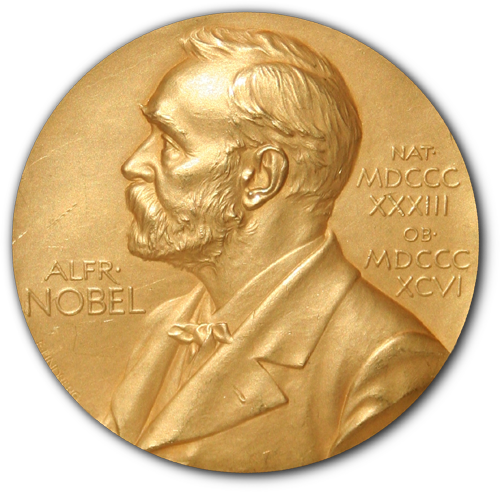
\includegraphics[width=0.8\linewidth]{figures/nobel.png}
    \par\vspace{0.2cm}
    \textbf{Physics Nobel Prize}
  \end{minipage}
\end{frame}


\begin{frame}{Formulations vs Interpretations}

  \begin{minipage}[t]{0.43\textwidth} % Columna izquierda
    \begin{block}{Formulations of Quantum Mechanics}
      \vspace{0.2cm}
      \begin{itemize}
        \item Heisenberg's Matrix Mechanics
        \item Schrödinger's Wave Mechanics
        \item Hilbert Space Formalism (von Neumann)
        \item Bohmian Mechanics (Wave function decomposition: $R$ and $S$)
      \end{itemize}
    \end{block}
  \end{minipage}
  \hfill
  \pause
  \begin{minipage}[t]{0.53\textwidth} % Columna derecha
    \begin{block}{Interpretations of Quantum Mechanics}
    \vspace{0.2cm}
      \begin{itemize}
        \item Copenhagen Interpretation (Statistical, Collapse of the wavefunction)
        \item EPR Argument and Reality Criterion
        \item de Broglie-Bohm Interpretation (Hidden Variables, Deterministic)
        \item Quantum Potential and Nonlocality
        \item Bell's Theorem (Incompatibility with Local Realism)
      \end{itemize}
    \end{block}
  \end{minipage}

\end{frame}


\begin{frame}{Mathematische Grundlagen der Quantenmechanik}
  \begin{minipage}{0.44\textwidth}
    \centering
    \tikz\node[draw=purple!50, fill=purple!10, rounded corners=5pt, drop shadow] {
      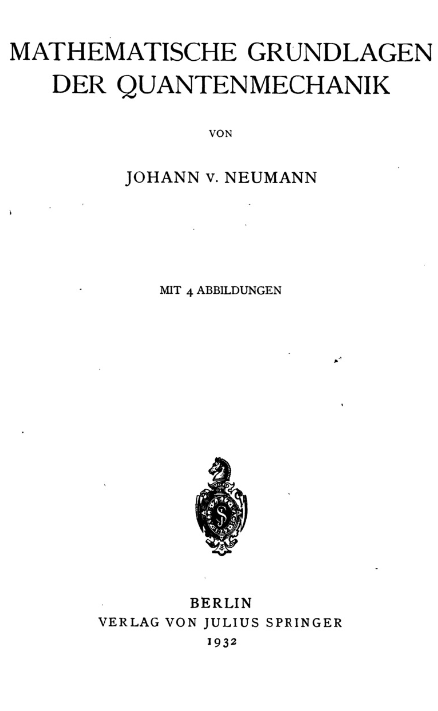
\includegraphics[width=0.6\linewidth]{figures/neumann1.png}
    };
    \par\vspace{0.2cm}
    \small \textit{First German edition (1932)}
 
  \end{minipage}
  \hfill
  \begin{minipage}{0.44\textwidth}
    \centering
    \tikz\node[draw=purple!50, fill=purple!10, rounded corners=5pt, drop shadow] {
      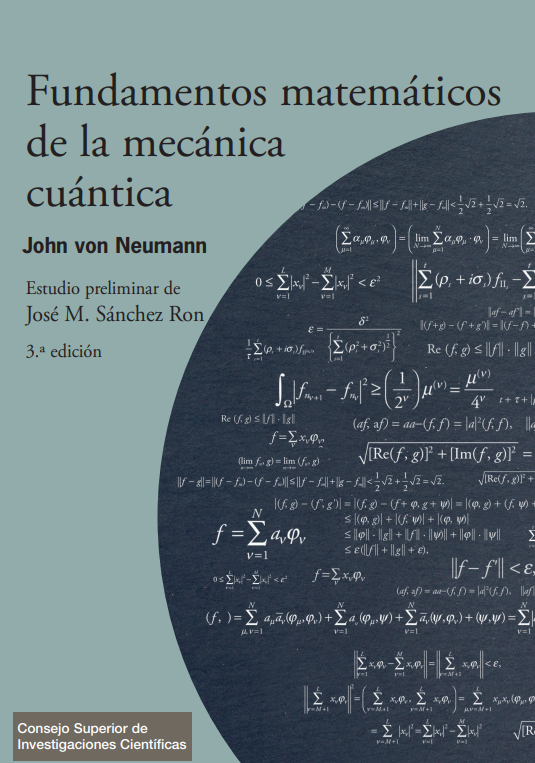
\includegraphics[width=0.65\linewidth]{figures/neumann2.png}
    };
    \par\vspace{0.2cm}
    \small \textit{Spanish translation (CSIC, 3rd edition)}

  \end{minipage}
\end{frame}

% Slide 1: Axioms
\begin{frame}{Von Neumann's Axioms (Section IV.1)}
  Von Neumann does not start from the quantum formalism itself, 
  but rather establishes general axioms for the mean value of any 
  physical magnitude $R$ in a statistical ensemble, denoted as $Vm(R)$.  

  \pause
  \begin{itemize}
    \item[A'.] \textbf{Positivity:}  
    If a magnitude $R$ is intrinsically non-negative (e.g. the square of another quantity), then  
    \[
    Vm(R) \geq 0
    \]

    \pause
    \item[B'.] \textbf{Linearity:}  
    For arbitrary magnitudes $R, S, \dots$ and real numbers $a, b, \dots$:  
    \[
    Vm(aR + bS + \dots) = aVm(R) + bVm(S) + \dots
    \]
  \end{itemize}
\end{frame}

% Slide 2: Statistical Operator
\begin{frame}{Statistical Operator and Impossibility Result (Section IV.2)}
 
  Von Neumann proves a fundamental theorem:  

  \pause
  Any expectation value function $Vm(R)$ that satisfies axioms A' and B' 
  can be uniquely represented by a Hermitian, positive operator $U$, 
  called the \textit{statistical operator} (today: density matrix), via the trace formula:

  \pause
  \[
    Vm(R) = \mathrm{Tr}(UR)
  \]
\end{frame}

\begin{frame}{Conditions for a Hidden-Variable System}
  In the hidden-variable hypothesis, any physical magnitude $R$ 
  must satisfy the following conditions:

  \pause
  \begin{enumerate}
    \item \textbf{Eigenvalue Condition:}  
    The expectation value of any magnitude $R$ must coincide with one of its possible values (eigenvalues).  
    \[
      Vm(R) \in \{\text{eigenvalues of } R\}
    \]

    \pause
    \item \textbf{Dispersion-Free Condition:}  
    The variance of any magnitude $R$ must vanish, i.e.  
    \[
      Vm(R^2) = [Vm(R)]^2
    \]
  \end{enumerate}
\end{frame}

\begin{frame}{Von Neumann's Impossibility Proof}
  The core of von Neumann's argument is to show that there is no statistical operator $U$ 
  (and therefore no expectation-value function $V_m(R)$) that can simultaneously satisfy 
  the linearity hypothesis (B') and the condition of absence of dispersion for all observables.

  \vspace{0.5cm}

  \[
    V_m(RS) + V_m(SR) = 2\,V_m(R)\,V_m(S)
  \]

  \vspace{0.5cm}

  For non-commuting observables ($[R,S]\neq 0$), there is in general no assignment 
  of values $V_m(\cdot)$ that can satisfy this for all operators.
\end{frame}



\begin{frame}{Bhom And Hidden Variables}
  % Minipages for the images
  \begin{minipage}{0.48\textwidth}
    \centering
    
\includegraphics[width=0.8\linewidth]{figures/einstein.jpeg}
    \par\vspace{0.2cm}
    \textbf{Albert Einstein}
  \end{minipage}
  \hfill
  \begin{minipage}{0.48\textwidth}
    \centering
    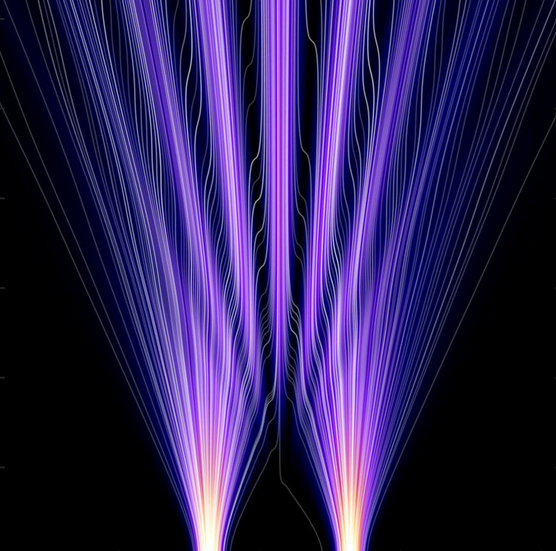
\includegraphics[width=0.9\linewidth]{figures/Bhom.png}
    \par\vspace{0.2cm}
    \textbf{Bhom Trayectories}
  \end{minipage}
\end{frame}


\begin{frame}{Bhom Hidden Variables Papers}
  \begin{minipage}{0.49\textwidth}
    \centering
    \tikz\node[draw=purple!50, fill=purple!10, rounded corners=5pt, drop shadow] {
      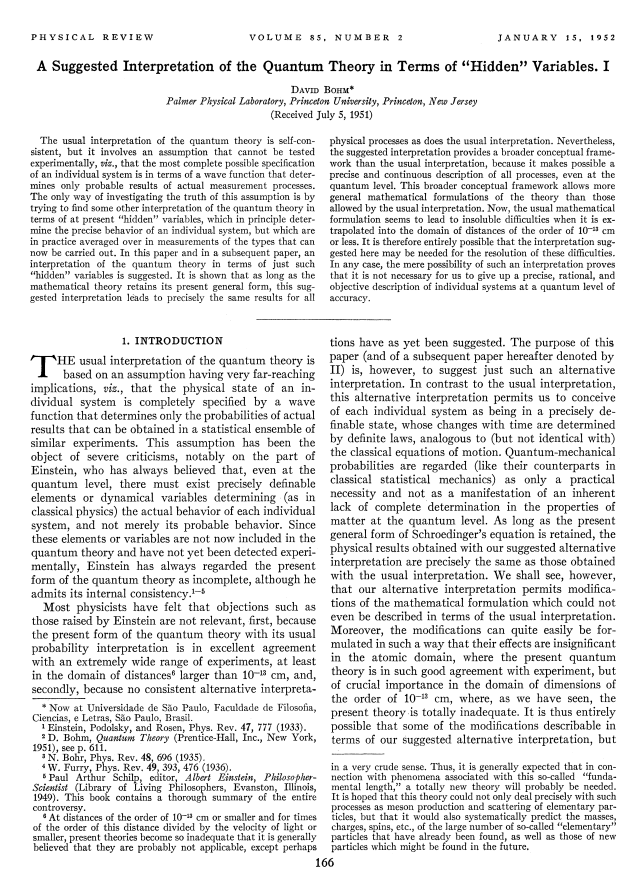
\includegraphics[width=0.7\linewidth]{figures/bhompaperI.png}
    };
    \par\vspace{0.2cm}
    \small \textit{Hidden Variable I (1951)}
 
  \end{minipage}
  \hfill
  \begin{minipage}{0.49\textwidth}
    \centering
    \tikz\node[draw=purple!50, fill=purple!10, rounded corners=5pt, drop shadow] {
      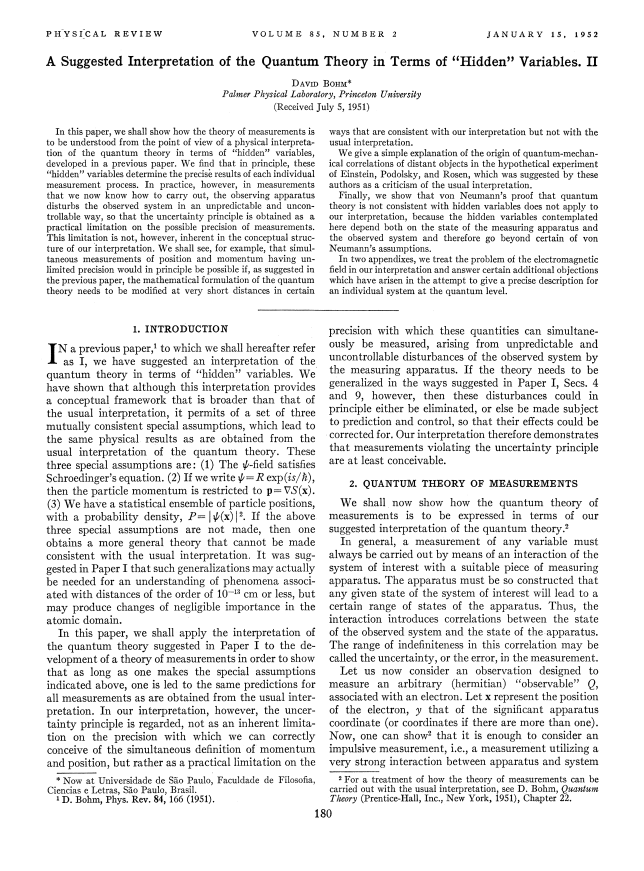
\includegraphics[width=0.7\linewidth]{figures/bhompaperII.png}
    };
    \par\vspace{0.2cm}
    \small \textit{Hidden Variables II (1951)}

  \end{minipage}
\end{frame}

%---------------------------------------------------------
\begin{frame}{Bohmian Mechanics: Wave Function in Polar Form}

  \textbf{Starting Point: Time-Dependent Schrödinger Equation}
  \[
    i\hbar \frac{\partial \psi}{\partial t} 
      = -\frac{\hbar^2}{2m}\nabla^2\psi + V(\mathbf{x},t)\psi
  \]

  \pause

  \textbf{Polar Decomposition of the Wave Function}
  \[
    \psi(\mathbf{x},t) = R(\mathbf{x},t)\,e^{\tfrac{i}{\hbar}S(\mathbf{x},t)}, 
    \quad R \geq 0,\; S\in \mathbb{R}
  \]

  \pause

  This representation will split Schrödinger’s equation into two coupled \emph{real} equations:  
  a continuity equation and a Hamilton–Jacobi–like equation.  

\end{frame}

%---------------------------------------------------------
\begin{frame}{Bohmian Mechanics: Continuity and Quantum Potential}

  \textbf{Continuity Equation (Probability Conservation)}
  \[
    \frac{\partial P}{\partial t} 
      + \nabla\!\cdot\!\big(P\,\tfrac{\nabla S}{m}\big) = 0, 
    \qquad P = R^2
  \]

  \pause

  \textbf{Modified Hamilton–Jacobi Equation}
  \[
    \frac{\partial S}{\partial t} 
      + \frac{(\nabla S)^2}{2m} 
      + V(\mathbf{x},t) 
      + U(\mathbf{x},t) = 0
  \]
\end{frame}
  

\begin{frame}{Bohmian Mechanics: Continuity, Quantum Potential and Motion}

  \textbf{Quantum Potential}
  \[
    U(\mathbf{x},t) = -\frac{\hbar^2}{2m}\,\frac{\nabla^2 R}{R}
  \]

  \pause

  \textbf{Guidance Equation (Deterministic Trajectories)}
  \[
    \mathbf{p} = \nabla S(\mathbf{x},t), 
    \qquad \mathbf{v} = \frac{\nabla S}{m}
  \]

  \pause

  \textbf{Equation of Motion (Newtonian Form with Quantum Force)}
  \[
    m \frac{d^2 \mathbf{x}}{dt^2} = - \nabla \Big( V(\mathbf{x}) + U(\mathbf{x},t) \Big)
  \]

\end{frame}



%---------------------------------------------------------
\begin{frame}{Statistical Predictions in Bohmian Mechanics}

  \textbf{Determinism vs. Statistics}


  Although Bohm’s theory is deterministic for single systems,  
  it reproduces all statistical predictions of standard quantum mechanics  
  under three key assumptions:

  \pause
  \begin{enumerate}
    \item The field $\psi$ satisfies the Schrödinger equation.  
    \pause
    \item The particle’s momentum is always given by $p = \nabla S(\mathbf{x})$.  
    \pause
    \item In practice, we cannot predict or control the exact initial position,  
          so we work with an ensemble with probability density:
          \[
            P(\mathbf{x}) = R^2 = |\psi(\mathbf{x})|^2
          \]
  \end{enumerate}

\end{frame}

%---------------------------------------------------------
\begin{frame}{Consistency of the Statistical Postulate}

  \textbf{Continuity Equation Ensures Born’s Rule Preservation}

  \pause
  Starting from the polar decomposition, the continuity equation is:
  \[
    \frac{\partial P}{\partial t} + \nabla \cdot (P \mathbf{v}) = 0,
    \qquad \mathbf{v} = \frac{\nabla S}{m}
  \]

  \pause
  This guarantees that if $P(\mathbf{x},t_0) = |\psi(\mathbf{x},t_0)|^2$  
  at one instant, then $P(\mathbf{x},t) = |\psi(\mathbf{x},t)|^2$  
  for all later times.

  \pause
  \textbf{Interpretation:}  
  Probability is not fundamental but reflects ignorance of initial conditions,  
  just as in classical statistical mechanics.  

\end{frame}


%---------------------------------------------------------
\begin{frame}{Quantum Potential in Many-Body Systems}

\textbf{Extension to $n$ particles}

\pause
For a system of $n$ particles, the wavefunction is:
\[
\psi(x_1, x_2, \dots, x_n, t) = R(x_1, \dots, x_n,t)\, e^{\tfrac{i}{\hbar} S(x_1, \dots, x_n,t)}
\]

\pause
The quantum potential generalizes to:
\[
U(x_1, \dots, x_n) \;=\; -\frac{\hbar^2}{2m} \, \frac{\sum_i \nabla_i^2 R}{R}
\]

\pause
\textbf{Key feature:} $U$ depends on the coordinates of \emph{all} particles simultaneously.  

\end{frame}

%---------------------------------------------------------
\begin{frame}{Nonlocality and Entanglement in Bohm's Theory}

\textbf{Implications of the many-body quantum potential:}


\begin{itemize}
  \item The force on particle $i$,
  \[
  \mathbf{F}_i = -\nabla_i U,
  \]
  depends instantaneously on the positions of all other particles.
  \pause
  \item This represents an effective "many-body force" that is inherently \textbf{nonlocal}.
  
  \item In entangled states, the correlations predicted by quantum mechanics emerge naturally from this nonlocal potential.
  
  \item Thus, Bohm’s theory is \textbf{causal but nonlocal}, consistent with the EPR scenario.
\end{itemize}

\end{frame}

\begin{frame}{Bell 1964 Paper}
  \begin{center}
    \tikz\node[draw=blue!50, fill=blue!10, rounded corners=5pt, drop shadow] {
      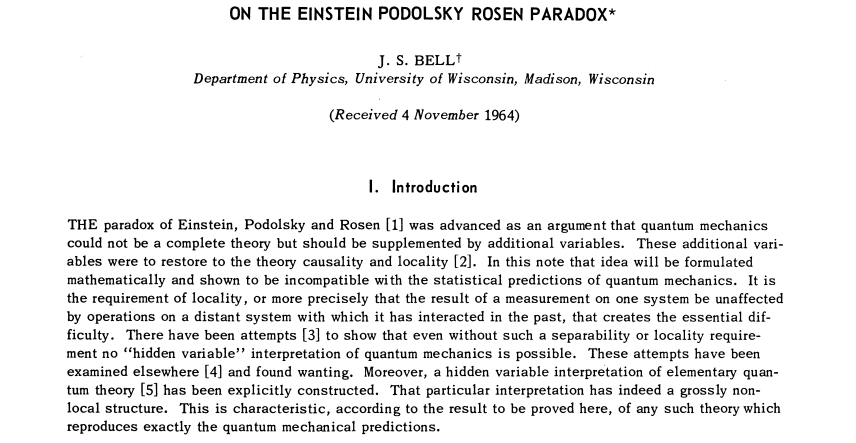
\includegraphics[width=0.8\linewidth]{figures/bell1964.png}
    };
    \par\vspace{0.3cm}
    \small \textit{On the Einstein Podolsky Rosen Paradox (1964)}
  \end{center}
\end{frame}

%---------------------------------------------------------
% SLIDE 1: Fundamental Assumptions by Bell
\begin{frame}{Fundamental Assumptions of Bell}

\begin{itemize}
  \item \textbf{Hidden variables:} Each particle pair has a set of parameters $\lambda$ that determines measurement outcomes locally. \pause
  \item \textbf{Measurement results:} $A(a,\lambda), B(b,\lambda) \in \{+1,-1\}$ represent outcomes along directions $a$ and $b$. \pause
  \item \textbf{Perfect anticorrelation:} If $a=b$, then $A(a,\lambda) = -B(a,\lambda)$, consistent with quantum prediction $P(a,a)=-1$. \pause
  \item \textbf{Local correlation:} 
  \[
    P(a,b) = \int d\lambda\, \rho(\lambda)\, A(a,\lambda) B(b,\lambda)
  \]
  where $\rho(\lambda)$ is the probability distribution over the hidden variables. \pause
  \item \textit{Interpretation: correlations are determined solely by local properties of the particles and their hidden variables.}
\end{itemize}

\end{frame}

%---------------------------------------------------------
% SLIDE 2: Intermediate Steps of the Derivation
\begin{frame}{Bell Derivation: Key Intermediate Steps}

\begin{enumerate}
  \item \textbf{Rewrite using anticorrelation:}  
  \[
    P(a,b) = - \int d\lambda\, \rho(\lambda) A(a,\lambda) A(b,\lambda)
  \]

  \item \textbf{Comparing three directions:}  
  \[
    P(a,b)-P(a,c) = - \int d\lambda\, \rho(\lambda) \big[ A(a)A(b) - A(a)A(c) \big]
  \] \pause

  \item \textbf{Regroup using $A(b)^2=1$:}  
  \[
    P(a,b)-P(a,c) = - \int d\lambda\, \rho(\lambda) A(a)A(b) \big[ 1 - A(b)A(c) \big]
  \] 
  \textit{The difference in correlations depends on how particle 2’s “instructions” change between $b$ and $c$.}
\end{enumerate}

\end{frame}

%---------------------------------------------------------
% SLIDE 3: Final Inequality and Physical Meaning
\begin{frame}{Bell Inequality and Physical Meaning}

\[
|P(a,b) - P(a,c)| \le 1 + P(b,c)
\] \pause

\begin{itemize}
  \item $P(a,b)$: correlation measured between results along $a$ and $b$. \pause
  \item $P(a,c)$: correlation measured between $a$ and $c$. \pause
  \item $P(b,c)$: correlation between directions $b$ and $c$. \pause
  \item \textbf{Physical interpretation:} No local realistic theory can produce correlations stronger than this bound. \pause
  \item Violation of this inequality by quantum predictions implies:
    \begin{itemize}
      \item Realism and locality cannot both hold simultaneously. 
      \item Measurement outcomes are correlated in a nonlocal manner via entanglement.
    \end{itemize}
\end{itemize}

\end{frame}

\begin{frame}{Violation of Bell Inequality: Quantum Prediction}

\textbf{Quantum mechanics prediction for entangled particles:}

\vspace{-0.3cm}

\[
P_\text{QM}(\mathbf{a}, \mathbf{b}) = - \mathbf{a} \cdot \mathbf{b}
\]
\vspace{-0.3cm}

\pause

\textbf{Bell inequality :}

\vspace{-0.3cm}

\[
|P(\mathbf{a},\mathbf{b}) - P(\mathbf{a},\mathbf{c})| \le 1 + P(\mathbf{b},\mathbf{c})
\]

\vspace{-0.3cm}

\pause

\textbf{Specific setup:}  
\begin{itemize}
  \item Take a vector $\mathbf{c}$ “halfway” between $\mathbf{a}$ and $\mathbf{b}$.  
  \item Define angles: 
  \(\theta = \angle(\mathbf{a},\mathbf{c}) = \angle(\mathbf{c},-\mathbf{b})\)
\end{itemize}

\pause

\textbf{Substituting the quantum prediction:}

\vspace{-0.3cm}

\[
|- \mathbf{a} \cdot \mathbf{b} - (- \mathbf{a} \cdot \mathbf{c})| 
\le 1 - \mathbf{c} \cdot \mathbf{b} 
\quad \Rightarrow \quad 
|\cos(2\theta) - \cos(\theta)| \le 1 - \cos(\theta)
\]

\end{frame}



\begin{frame}{Explicit Violation for Small Angles}

\textbf{Approximations for small angles $\theta \ll 1$:}
\[
\cos(\theta) \approx 1 - \frac{\theta^2}{2}, \quad 
\cos(2\theta) \approx 1 - 2\theta^2
\]

\pause

\textbf{Bell inequality becomes:}
\[
| \cos(2\theta) - \cos(\theta) | \le 1 - \cos(\theta)
\quad \Rightarrow \quad
|(1 - 2\theta^2) - (1 - \frac{\theta^2}{2})| \le \frac{\theta^2}{2}
\]

\pause

\textbf{Simplifying:}
\[
\frac{3}{2}\theta^2 \le \frac{1}{2} \theta^2
\]

\pause

\textbf{Conclusion:}  
This inequality is \textbf{false} for any $\theta \neq 0$, demonstrating that 
\textbf{quantum mechanics predictions violate Bell’s inequality}.  

\end{frame}


\begin{frame}{Bell’s Refutation of von Neumann (1966)}

\begin{minipage}{0.65\textwidth}
\textbf{Bell’s Conceptual Criticism:}
\begin{itemize}
  \item Von Neumann’s \textbf{linearity assumption}: 
   \vspace{-0.4cm}

  \[
    V_m(aR+bS) = aV_m(R) + bV_m(S)
  \]

  \vspace{-0.3cm}
  \pause
  \item Imposed even on dispersion-free states.  
  \pause
  \item Bell argued this is \textbf{unjustified for non-commuting observables}.  
  \pause
  \item Example: measuring $\sigma_x + \sigma_y$ is not the same as separately measuring $\sigma_x$ and $\sigma_y$.  
  \pause
  \item Therefore, von Neumann’s proof excludes only a very restrictive class of hidden-variable theories.  
  \pause
  \item Bohm’s 1952 theory escapes because it is \textbf{contextual}.  
\end{itemize}
\end{minipage}
\hfill
\begin{minipage}{0.33\textwidth}
  \centering

  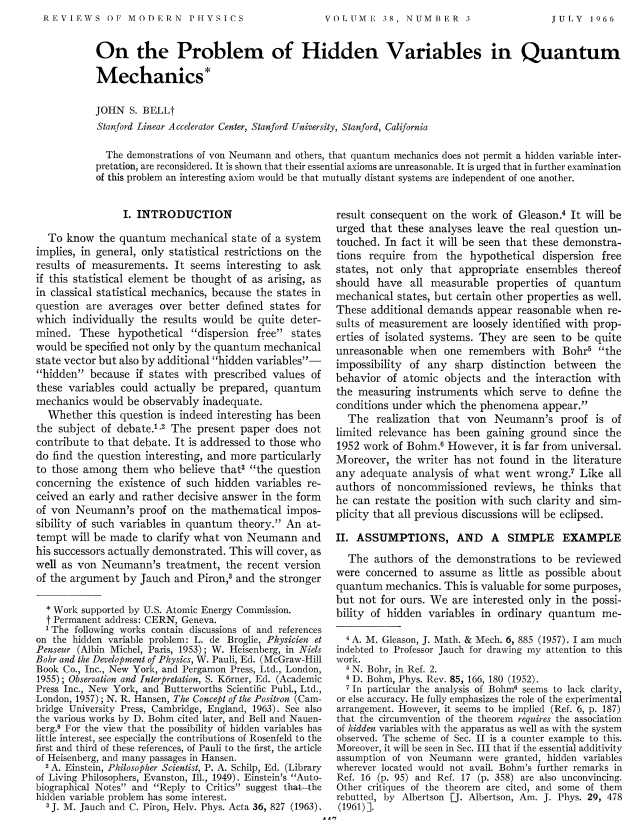
\includegraphics[width=\textwidth]{figures/bell1966.png} \\
  \vspace{0.2cm}
  {\footnotesize Bell, J.S. \\
  \emph{On the problem of hidden variables in QM} (1966)}
\end{minipage}

\end{frame}




\begin{frame}{The CHSH Inequality}

\begin{minipage}{0.58\textwidth}

\textbf{Defining the correlation function:}

\vspace{-0.5cm}

\[
E(a,b) = \langle A(a) \, B(b) \rangle, 
\quad A, B = \pm 1
\]

\pause

\vspace{-0.2cm}

\textbf{The CHSH combination:}

\vspace{-0.6cm}

\[
S = E(a, b) - E(a, b') + E(a', b) + E(a', b')
\]

\pause

\vspace{-0.3cm}

\textbf{Local realism constraint:}

\vspace{-0.5cm}

\[
-2 \leq S \leq 2
\]

\pause

\vspace{-0.3cm}

\textbf{Quantum mechanics prediction:}

\vspace{-0.6cm}

\[
|S| \leq 2\sqrt{2} \quad \Rightarrow \quad \text{Violation of local realism}
\]

\pause

\vspace{-0.3cm}


\textbf{Impact:}
\begin{itemize}
  \item The CHSH form was \textbf{experimentally testable}.  
  \item Enabled landmark tests (e.g. Aspect, 1982).  
\end{itemize}

\end{minipage}
\hfill
\begin{minipage}{0.36\textwidth}

\textbf{Why correlations matter:}

\begin{itemize}
  \item The values $E(a,b)$ come from \textbf{statistical counts} of coincident detections.  
  \item Individual outcomes are random, but correlations reveal hidden structure.  
  \item The strength of violation depends entirely on these \textbf{count-based correlations}.  
\end{itemize}

\end{minipage}

\end{frame}



\begin{frame}{Conclusions on Quantum Entanglement}

\begin{itemize}
  \item EPR raised the dilemma about the \textbf{completeness} of quantum mechanics.  
  \pause
  \item Bell turned the \textbf{philosophical} debate into \textbf{mathematical and experimental predictions}.  
  \pause

  \item Entanglement reveals \textbf{nonlocal correlations}.  
  \pause
  \item Incompatible with classical \textbf{realism} and \textbf{locality}.  
\end{itemize}

\end{frame}




\section{Mathematical Framework for Entanglement}
\label{sec:math_framework}

Although quantum entanglement first emerged as a mathematical feature of the
early formulations of quantum mechanics, subsequent experimental confirmations
and theoretical advancements have enabled a more rigorous description.
The core of this description lies in how we represent the state of a
composite quantum system. While the framework is well-established, its
physical interpretation---a common theme in quantum theory---remains a
subject of active debate.

\subsection{Departure from Classical State Spaces}
\label{sub:departure_classical}

In any formalism of classical mechanics (e.g., Hamiltonian), the state of a
composite system is constructed from the states of its individual parts.
For a two-particle system, $A$ and $B$, the total state is a point
$(x_A, x_B)$ in the Cartesian product of the individual
phase spaces, $\Gamma_{AB} = \Gamma_A \times \Gamma_B$.
Here, $x_i = (q_i, p_i)$ represents the generalized coordinates and
momenta for particle $i$. This structure implies that specifying the state of
each subsystem completely specifies the state of the whole.

A naive extrapolation to quantum mechanics would suggest that the state space
of a two-particle system is the Cartesian product of the individual Hilbert
spaces, $\mathcal{H}_{AB} = \mathcal{H}_A \times \mathcal{H}_B$. However, this
structure is insufficient because it fails to incorporate the
superposition principle correctly. A state in
$\mathcal{H}_A \times \mathcal{H}_B$ is an ordered pair $(\ket{\psi_A},
\ket{\phi_B})$, but this framework does not naturally accommodate the
linear combinations of such pairs that are physically essential.

To resolve this, the state space for a composite quantum system is
constructed using the tensor product of the individual Hilbert
spaces:
\begin{equation}
	\mathcal{H}_{AB} = \mathcal{H}_A \otimes \mathcal{H}_B.
\end{equation}
A general pure state $\ket{\Psi}$ in this composite space is a superposition
of basis states:
\begin{equation}
	\ket{\Psi} = \sum_{i,j} c_{ij} (\ket{a_i} \otimes \ket{b_j}),
	\label{eq:general_state}
\end{equation}
where $\{\ket{a_i}\}$ and $\{\ket{b_j}\}$ are orthonormal bases for
$\mathcal{H}_A$ and $\mathcal{H}_B$, respectively. The dimension of this new
space is the product of the dimensions of the constituent spaces,
$\dim(\mathcal{H}_{AB}) = \dim(\mathcal{H}_A) \cdot \dim(\mathcal{H}_B)$.

\subsection{Separable and Entangled States}
\label{sub:separable_entangled}

The structure of the tensor product space $\mathcal{H}_{AB}$ allows for two
fundamentally different classes of states.

\paragraph{Separable States.}
A state is called separable (or a product state) if it
can be written as a single tensor product of states from the subsystems,
i.e.,
\begin{equation}
	\ket{\Psi}_{\text{sep}} = \ket{\psi_A} \otimes \ket{\psi_B},
\end{equation}
where $\ket{\psi_A} \in \mathcal{H}_A$ and $\ket{\psi_B} \in \mathcal{H}_B$.
For these states, the subsystems have definite individual properties,
independent of one another, analogous to the classical case.

\paragraph{Entangled States.}
If a state $\ket{\Psi} \in \mathcal{H}_{AB}$ cannot be written in the
separable form above, it is called an entangled state. These states
represent a uniquely quantum-mechanical correlation between subsystems.
Measuring a property of subsystem $A$ instantaneously influences the
properties of subsystem $B$, regardless of the physical distance
separating them.

\subsection{Operators and the Density Matrix Formalism}
\label{sub:operators_density}

An operator $O_A$ acting only on subsystem $A$ is represented on the
composite space as $O_A \otimes I_B$, where $I_B$ is the
identity operator on $\mathcal{H}_B$. Such operators are called
local operators. A general operator on $\mathcal{H}_{AB}$ is a
linear combination of tensor products of local operators.

The inner product on $\mathcal{H}_{AB}$ is defined by extending the inner
products of the subsystems linearly:
\begin{equation}
	(\bra{\phi_A} \otimes \bra{\phi_B}) (\ket{\psi_A} \otimes \ket{\psi_B})
	= \braket{\phi_A | \psi_A}_{\mathcal{H}_A} \braket{\phi_B | \psi_B}_{\mathcal{H}_B}.
\end{equation}

While pure states $\ket{\Psi}$ describe systems with maximal information,
entanglement forces us to consider situations of incomplete information,
especially when looking at only one part of an entangled pair. The
density matrix (or density operator), $\rho$, provides the necessary
formalism.

For a pure state $\ket{\Psi}$, the density matrix is the projection operator:
\begin{equation}
	\rho_{\text{pure}} = \ket{\Psi}\bra{\Psi}.
\end{equation}
A key property of a pure state's density matrix is that it is a projector,
meaning $\rho^2 = \rho$. This leads to a simple test for purity:
\begin{equation}
	\mathrm{Tr}(\rho^2) = 1,
\end{equation}
where the value $\mathrm{Tr}(\rho^2)$ is known as the \textit{purity} of the
state.

If we have statistical knowledge of a system (an ensemble of pure states
$\{\ket{\psi_i}\}$ with probabilities $\{p_i\}$), the state is a
mixed state, described by the density matrix:
\begin{equation}
	\rho_{\text{mixed}} = \sum_i p_i \ket{\psi_i}\bra{\psi_i}.
\end{equation}
For any mixed state, the purity is less than one:
$\mathrm{Tr}(\rho_{\text{mixed}}^2) < 1$.

\subsection{Quantifying Uncertainty: Von Neumann Entropy}
\label{sub:von_neumann_entropy}

The density matrix allows us to assign a single number to quantify the
degree of uncertainty or ``mixedness'' of a quantum state. This measure is the
Von Neumann entropy, defined as:
\begin{equation}
	S(\rho) = - \mathrm{Tr}(\rho \ln \rho).
\end{equation}
This is the quantum mechanical analogue of the Gibbs entropy in statistical
mechanics. If the eigenvalues of $\rho$ are $\lambda_i$, the entropy can be
calculated as $S = - \sum_i \lambda_i \ln \lambda_i$.

The Von Neumann entropy has several key properties:
\begin{itemize}
	\item For any pure state, $\rho = \ket{\psi}\bra{\psi}$, the
		entropy is zero, $S(\rho) = 0$. This corresponds to a state of
		maximal knowledge or zero uncertainty.
	\item For a maximally mixed state in a $d$-dimensional Hilbert
		space, where $\rho = I/d$, the entropy is maximal,
		$S(\rho) = \ln d$. This corresponds to a state of minimal knowledge.
\end{itemize}

The true power of this measure becomes apparent when applied to entangled
systems. Consider a composite system $AB$ in a pure state
$\ket{\Psi}_{AB}$, for which $S(\rho_{AB})=0$. If we are interested only in
subsystem $A$, its state is described by the reduced density matrix,
$\rho_A$, obtained by tracing over subsystem $B$:
\begin{equation}
	\rho_A = \mathrm{Tr}_B(\rho_{AB}) = \mathrm{Tr}_B(\ket{\Psi}_{AB}\bra{\Psi}_{AB}).
\end{equation}
If the global state $\ket{\Psi}_{AB}$ is entangled, the local state $\rho_A$
will be a mixed state, and its entropy $S(\rho_A)$ will be greater than zero.
This non-zero entropy of a subsystem, despite the global system being in a
pure state, is a fundamental signature of entanglement. For any pure
bipartite state, $S(\rho_A) = S(\rho_B)$, and this value is used as the
entropy of entanglement.

\section{Quantifying and Detecting Entanglement}
\label{sec:quantifying_detecting}

With the mathematical framework established, we need tools to answer two
practical questions: How much entanglement does a state possess? And how can
we experimentally detect it, especially in mixed states?

\subsection{Pure States: Schmidt Decomposition and Entropy of Entanglement}
\label{sub:pure_state_measures}

For pure bipartite states, a powerful theorem known as the
Schmidt decomposition provides a canonical form. Any state
$\ket{\Psi}_{AB}$ can be written as a single sum:
\begin{equation}
	\ket{\Psi}_{AB} = \sum_{k=1}^{r_S} \sqrt{\lambda_k} \ket{k}_A \otimes \ket{k}_B,
\end{equation}
where $\{\ket{k}_A\}$ and $\{\ket{k}_B\}$ are orthonormal bases for their
respective subsystems, and $\lambda_k > 0$ with $\sum_k \lambda_k = 1$. The
number of terms, $r_S$, is the Schmidt rank. A state is separable if
and only if its Schmidt rank is 1.

The degree of entanglement is uniquely quantified by the
entropy of entanglement. This is simply the Von Neumann entropy of
the reduced density matrix of either subsystem:
\begin{equation}
	E(\ket{\Psi}) = S(\rho_A) = -\mathrm{Tr}(\rho_A \ln \rho_A) = -\sum_{k=1}^{r_S} \lambda_k \ln \lambda_k.
\end{equation}
The Schmidt coefficients $\sqrt{\lambda_k}$ are directly related to the
eigenvalues of the reduced density matrix, elegantly connecting the
state's structure to its entanglement content.

\subsection{Mixed States: A Zoo of Measures}
\label{sub:mixed_state_measures}
Quantifying entanglement in mixed states is far more complex, as they lack
a unique decomposition. Several measures exist, each with a different
operational or geometric motivation.

\paragraph{Entanglement of Formation ($E_F$).}
This measure asks: what is the minimum average entanglement (of pure states)
required to create a given mixed state $\rho$? It is defined via a
``convex roof'' construction:
\begin{equation}
	E_F(\rho) = \min_{\{p_i, \ket{\psi_i}\}} \sum_i p_i E(\ket{\psi_i}),
\end{equation}
where the minimization is over all possible pure-state ensembles
$\{p_i, \ket{\psi_i}\}$ that decompose $\rho$.

\paragraph{Concurrence ($C$).}
For the specific case of two-qubit systems, the Concurrence is a widely
used measure computationally related to $E_F$. It has the great advantage
of having a closed-form analytical solution, making it highly practical.

\paragraph{Relative Entropy of Entanglement ($E_R$).}
This measure takes a geometric approach, defining the entanglement of a
state $\rho$ as its ``distance'' to the set of all separable states (SEP):
\begin{equation}
	E_R(\rho) = \min_{\sigma \in \text{SEP}} S(\rho || \sigma),
\end{equation}
where $S(\rho || \sigma) = \mathrm{Tr}(\rho \ln \rho - \rho \ln \sigma)$ is
the quantum relative entropy.

\subsection{Detecting Mixed-State Entanglement}
\label{sub:detecting_entanglement}
Distinguishing a separable mixed state from an entangled one is a major
challenge. Several criteria have been developed.

\paragraph{The PPT Criterion.}
A simple but powerful test is the Positive Partial Transpose (PPT)
criterion. If a state $\rho_{AB}$ is separable, then its partial transpose
with respect to one subsystem, $\rho^{T_B}$, must be a valid (positive
semidefinite) density matrix. While this is a necessary condition for
separability in all dimensions, it is only a sufficient one for
$2 \times 2$ and $2 \times 3$ systems. The degree to which a state fails
this test can be quantified by a measure called Negativity.

\paragraph{Worked Example: The Werner State.}
To make this concrete, let's analyse a two-qubit Werner state, a mixture
of a maximally entangled Bell state and a maximally mixed state. Using the
singlet state $\ket{\Psi^-} = \frac{1}{\sqrt{2}}(\ket{01}-\ket{10})$, the
Werner state is defined for $p \in [0, 1]$ as:
\begin{equation}
	\rho_W = p \ket{\Psi^-}\bra{\Psi^-} + \frac{1-p}{4} \mathbb{I}_4.
\end{equation}
In the computational basis $\{\ket{00}, \ket{01}, \ket{10}, \ket{11}\}$, this is:
\begin{equation}
	\rho_W = \frac{1}{4}
	\begin{pmatrix}
		1-p & 0 & 0 & 0 \\
		0 & 1+p & -2p & 0 \\
		0 & -2p & 1+p & 0 \\
		0 & 0 & 0 & 1-p
	\end{pmatrix}.
\end{equation}
We apply the partial transpose to the second qubit (subsystem B):
\begin{equation}
	\rho_W^{T_B} = \frac{1}{4}
	\begin{pmatrix}
		1-p & 0 & 0 & -2p \\
		0 & 1+p & 0 & 0 \\
		0 & 0 & 1+p & 0 \\
		-2p & 0 & 0 & 1-p
	\end{pmatrix}.
\end{equation}
The state is entangled if this matrix has a negative eigenvalue. The four
eigenvalues of $\rho_W^{T_B}$ are found to be:
\begin{equation}
	\lambda_{1,2,3} = \frac{1+p}{4}, \quad \lambda_4 = \frac{1-3p}{4}.
\end{equation}
The first three are always non-negative for $p \in [0,1]$. However,
$\lambda_4$ becomes negative if $1-3p < 0$, which means $p > 1/3$.
Therefore, the Werner state is entangled for $p > 1/3$. The Negativity for
this state is the absolute value of the single negative eigenvalue:
\begin{equation}
	\mathcal{N}(\rho_W) = \max\left(0, -\lambda_4\right) = \max\left(0, \frac{3p-1}{4}\right).
\end{equation}

\paragraph{Entanglement Witnesses.}
An entanglement witness is a Hermitian operator $W$ that acts as a
detector. It is constructed such that its expectation value is non-negative
for all separable states but can be negative for at least one entangled state:
\begin{itemize}
	\item $\mathrm{Tr}(W \rho_{\text{sep}}) \ge 0$ for all $\rho_{\text{sep}} \in \text{SEP}$.
	\item If one measures $\mathrm{Tr}(W \rho) < 0$, the state $\rho$ is certified as entangled.
\end{itemize}
Geometrically, $W$ defines a hyperplane that separates a specific entangled
state from the convex set of separable states, making it a targeted tool for
experimental detection.

\section{Alternative Perspectives}
\label{sec:alternative_perspectives}

While the Hilbert space formalism is the standard, alternative mathematical
frameworks offer different physical insights. One such approach is through
Geometric Algebra, which interprets entanglement not as an intrinsic
property of a state, but as a relationship between reference frames, described
by a superposition of relative rotations. This shifts the focus from analysing
states to analysing the fundamental transformation operators themselves.


\section{Experimental Proofs}
% --- SLIDE 22: CHSH Inequality ---
\begin{frame}{The Bridge to Reality: The CHSH Inequality}
  
  \begin{block}{From Theory to Practice}
    \begin{itemize}[<+->]
      \item The CHSH inequality was the key theoretical tool that allowed for the design of the Freedman and Clauser experiment.
    \end{itemize}
  \end{block}
  
  \begin{alertblock}{The Decisive Inequality ($\delta$)}
    \justifying
    For the angles of predicted maximum violation ($\phi=22.5^\circ$ and $3\phi=67.5^\circ$), the inequality was simplified to a single expression:
    $$ \delta = \frac{R(22.5^\circ)}{R_0} - \frac{R(67.5^\circ)}{R_0} - \frac{1}{4} $$
    \begin{itemize}[<+->]
        \item \textbf{Local Realism} requires: $\boldsymbol{\delta \le 0}$
        \item \textbf{Quantum Mechanics} predicts: $\boldsymbol{\delta > 0}$
    \end{itemize}
  \end{alertblock}

\end{frame}

% --- SLIDE 23: Photon Source ---
\begin{frame}{Photon Source: Calcium Atomic Cascade}
  
  \begin{block}{Generating Entangled Pairs}
    \begin{itemize}[<+->]
      \item An atomic cascade in calcium atoms was used to generate photon pairs.
      \item The \textbf{J=0 $\rightarrow$ J=1 $\rightarrow$ J=0} transition emits two photons.
      \item By conservation of angular momentum, the photons' polarizations are strongly \textbf{correlated} (parallel).
    \end{itemize}
  \end{block}

\end{frame}

% --- SLIDE 24: Apparatus ---
\begin{frame}{Optical and Detection Apparatus}
  
  \begin{columns}[T]
    \begin{column}{0.6\textwidth}
      \begin{block}{Key Measurement Components}
        \begin{itemize}[<+->]
          \item The optical system used lenses, filters, and \textbf{``pile-of-plates'' polarizers}.
          \item The detectors were high-sensitivity \textbf{photomultiplier tubes (PMTs)}.
          \item The overall detection efficiency was extremely low ($\approx 1.6 \times 10^{-3} $), requiring long hours of measurement.
        \end{itemize}
      \end{block}
    \end{column}
    
    \begin{column}{0.4\textwidth}
      \begin{figure}
        \centering
        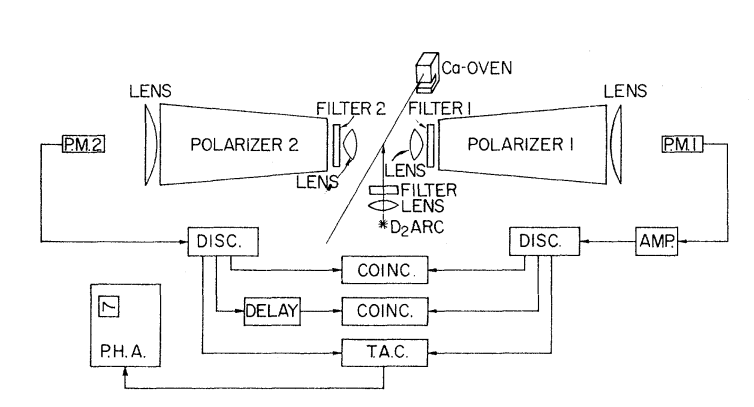
\includegraphics[width=\linewidth, height=0.7\textheight, keepaspectratio]{images/clauster.png}
        \caption{Scheme of the experimental setup \cite{freedman_experimental_1972}.}
      \end{figure}
    \end{column}
  \end{columns}

\end{frame}

% --- SLIDE 25: Results and Loopholes ---
\begin{frame}{Results, Verdict, and Loopholes}
  
  \begin{block}{Protocol and Result}
    \begin{itemize}[<+->]
      \item The experiment lasted approximately \textbf{200 hours} due to the low coincidence rate.
      \item A robust real-time normalization system was used to cancel out equipment drift.
    \end{itemize}
  \end{block}
  
  \begin{alertblock}<3->{The Decisive Experimental Result}
    \centering
    The measured value was:
    $\delta = 0.050 \pm 0.008$
  \end{alertblock}
  \pause

  \begin{block}<5->{Required Improvements: The Loopholes}
    \begin{itemize}[<+->]
      \item Despite its success, the experiment was not airtight:
      \begin{itemize}
          \item \textbf{Locality Loophole:} The polarizers could, in theory, ``communicate''. (Closed by Aspect in the 80s).
          \item \textbf{Detection Loophole:} The low efficiency could have biased the sample of detected pairs. (Closed in more recent experiments).
      \end{itemize}
    \end{itemize}
  \end{block}

\end{frame}


\section{Aspect and team}
\begin{frame}{Clauser--Horne 1974 Paper}
  \begin{center}
    \tikz\node[draw=red!50, fill=red!10, rounded corners=5pt, drop shadow] {
      \includegraphics[width=0.9\linewidth]{images/ch.png}
    };
    \par\vspace{0.3cm}
    \small \textit{Clauser \& Horne: Experimental Consequences of Objective Local Theories (1974)}
  \end{center}
\end{frame}





\begin{frame}{Clauser--Horne Formulation (1974)}

\begin{itemize}
  \item Defined \textbf{Objective Local Theories (OLT)}:  
        outcomes depend only on hidden variables $\lambda$ and local settings, not on distant settings.  
  \pause
  \item Introduced the \textbf{No-Enhancement Assumption}:  
        detection with a polarizer cannot exceed detection without it.  
  \pause
  \item Showed that this weaker assumption was still enough to make Freedman--Clauser results incompatible with all OLT satisfying it.  
  \pause
  \item Proved that some \textbf{supplementary assumption is necessary}:  
        without no-enhancement, one can build an OLT reproducing quantum predictions.  
  \pause
  \item Revealed the \textbf{detection loophole}:  
        experiments of that era only excluded OLT within the no-enhancement class.  
\end{itemize}

\end{frame}


\begin{frame}{Aspect's Experimental Setups (1980s)}

\begin{minipage}{0.58\textwidth}
\vspace{-2.cm}
\textbf{Experimental Program:}
\begin{itemize}
  \item Systematic tests of Bell inequalities using entangled photons from a calcium cascade.  
  \item Progressively designed to close detection and locality loopholes.  
\end{itemize}

\pause

\textbf{Key Features:}
\begin{itemize}
  \item 1981: High-efficiency source, single-channel polarizers.  
  \item 1982 (Two-channel): Polarizing beam splitters, closed the detection loophole.  
  \item 1982 (Time-varying analyzers): Fast switches, addressed the locality loophole.  
\end{itemize}

\vspace{-0.8cm}

\end{minipage}
\hfill
\begin{minipage}{0.38\textwidth}
  \centering
  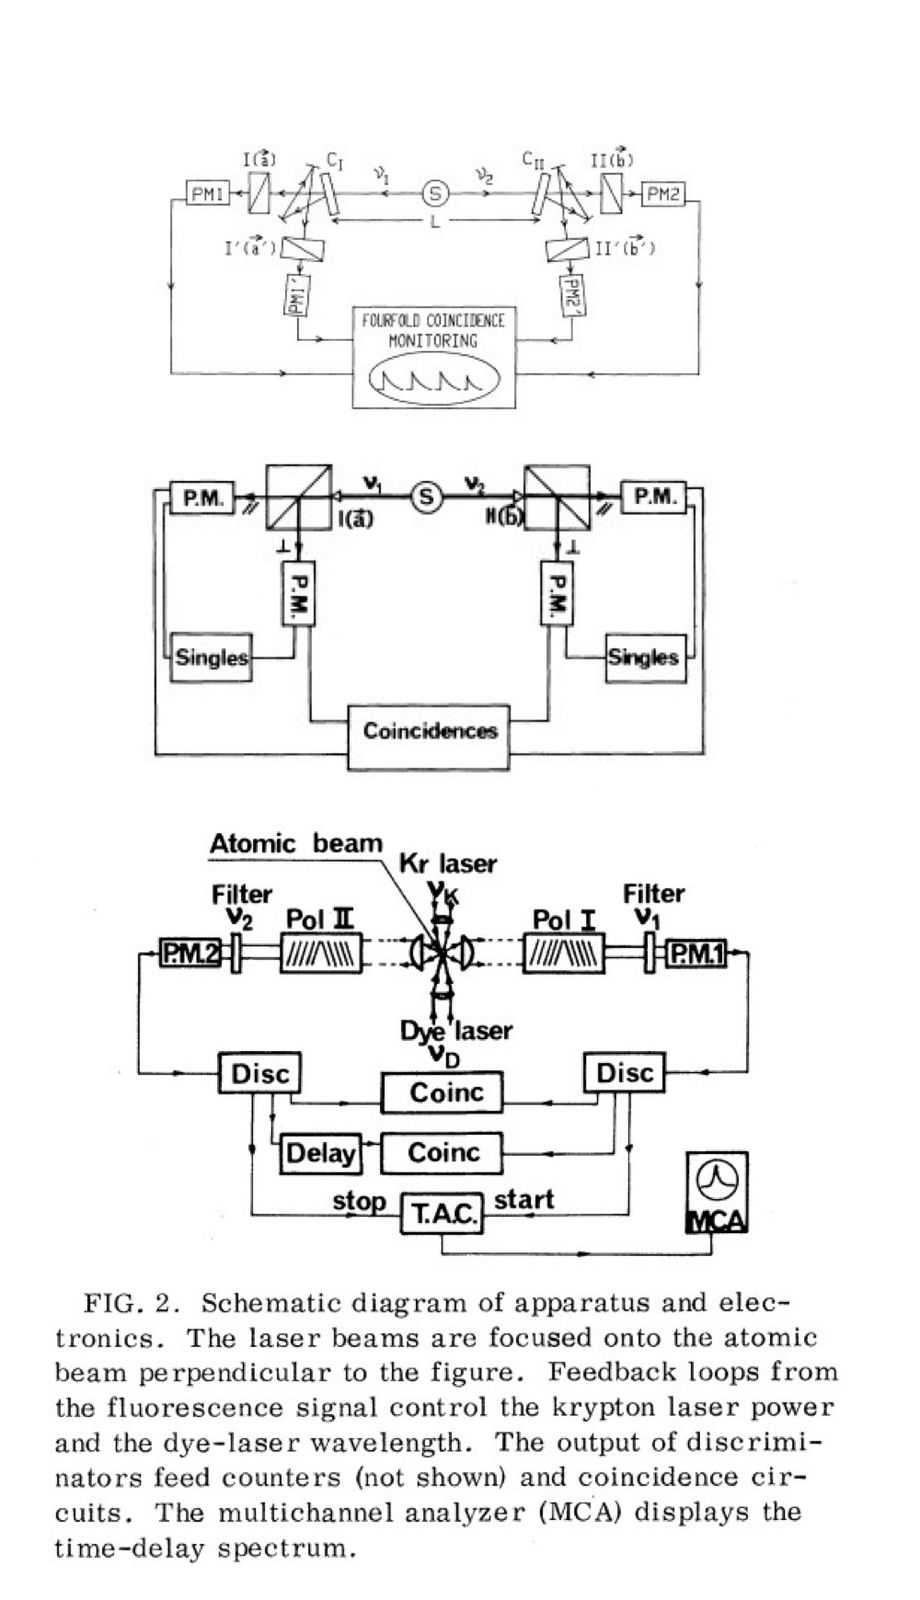
\includegraphics[width=0.8\linewidth]{images/aspect.jpeg} % <--- Imagen del montaje
  \par\vspace{0.2cm}
  \small \textit{Aspect’s photon cascade experiment.}
\end{minipage}

\end{frame}


\begin{frame}{Comparing Aspect’s Three Experiments}

\begin{block}{Progression of Experimental Design}
\begin{itemize}
  \item \textbf{1981:} Improved Freedman–Clauser setup, but still relied on \textit{no-enhancement} assumption (detection loophole).  
  \pause
  \item \textbf{1982 (Two-channel):} Stern–Gerlach–like measurement with PBS. Closed the detection loophole via \textit{fair sampling} assumption.  
  \pause
  \item \textbf{1982 (Time-varying analyzers):} Fast switches ensured space-like separation of choices. Closed the \textit{locality loophole}.  
\end{itemize}
\end{block}

\pause

\begin{center}
  \textbf{Impact:} Each step addressed a loophole, making the violation of Bell’s inequalities increasingly robust and conclusive.  
\end{center}

\end{frame}




\section{Applications}
% --- SLIDE 26: Applications (I) ---
\begin{frame}{Applications of Quantum Entanglement (I)}

  \begin{block}{1. Quantum Computing}
    \begin{itemize}[<+->]
      \item Entangled \textbf{qubits} are the foundation of quantum computers.
      \item They allow for computations impossible for classical computers.
      \item Advances in cryptography, drug discovery, and materials science.
    \end{itemize}
  \end{block}

  \begin{alertblock}{2. Quantum Cryptography (QKD)}
    \begin{itemize}[<+->]
      \item Uses pairs of entangled photons to generate cryptographic keys.
      \item Offers \textbf{unconditional security} (guaranteed by the laws of physics).
      \item Any eavesdropping attempt disturbs the entanglement and is detected.
    \end{itemize}
  \end{alertblock}

\end{frame}

% --- SLIDE 27: Applications (II) ---
\begin{frame}{Applications of Quantum Entanglement (II)}

  \begin{block}{3. Quantum Communication and Networks}
    \begin{itemize}[<+->]
      \item Foundation for a future \textbf{quantum internet}.
      \item Enables hyper-secure communications and the interconnection of distributed quantum computers.
      \item Development of quantum repeaters for long distances.
    \end{itemize}
  \end{block}

  \begin{alertblock}{4. Quantum Metrology and Sensing}
    \begin{itemize}[<+->]
      \item Creates \textbf{sensors much more sensitive} than classical physics allows.
      \item Allows for measurements with precision beyond the ``standard quantum limit''.
      \item Applications in atomic clocks, GPS, weak-field detection, and microscopy.
    \end{itemize}
  \end{alertblock}

\end{frame}

% --- SLIDE 28: Applications (III) ---
\begin{frame}{Applications of Quantum Entanglement (III)}

  \begin{block}{5. Quantum Simulation and Teleportation}
    \begin{itemize}[<+->]
      \item \textbf{Quantum Simulation:} Modeling complex systems (molecules, materials) impossible for classical computers.
      \item \textbf{Quantum Teleportation:} Transferring quantum states (information) between distant particles.
    \end{itemize}
  \end{block}

\end{frame}


\section{References}
\begin{frame}[allowframebreaks]{References}
	\printbibliography
	\nocite{*}
\end{frame}

\begin{frame}[plain]
	\centering
	\vspace{1cm}
	{\Huge \textbf{Thank you!}}\\[1cm]
	{\large Questions or Comments?}
\end{frame}

\begin{frame}
	\titlepage
\end{frame}

\end{document}
